\section{Athena Demonstration}
\label{sec-demo}

\begin{figure*}[tp]
\centering
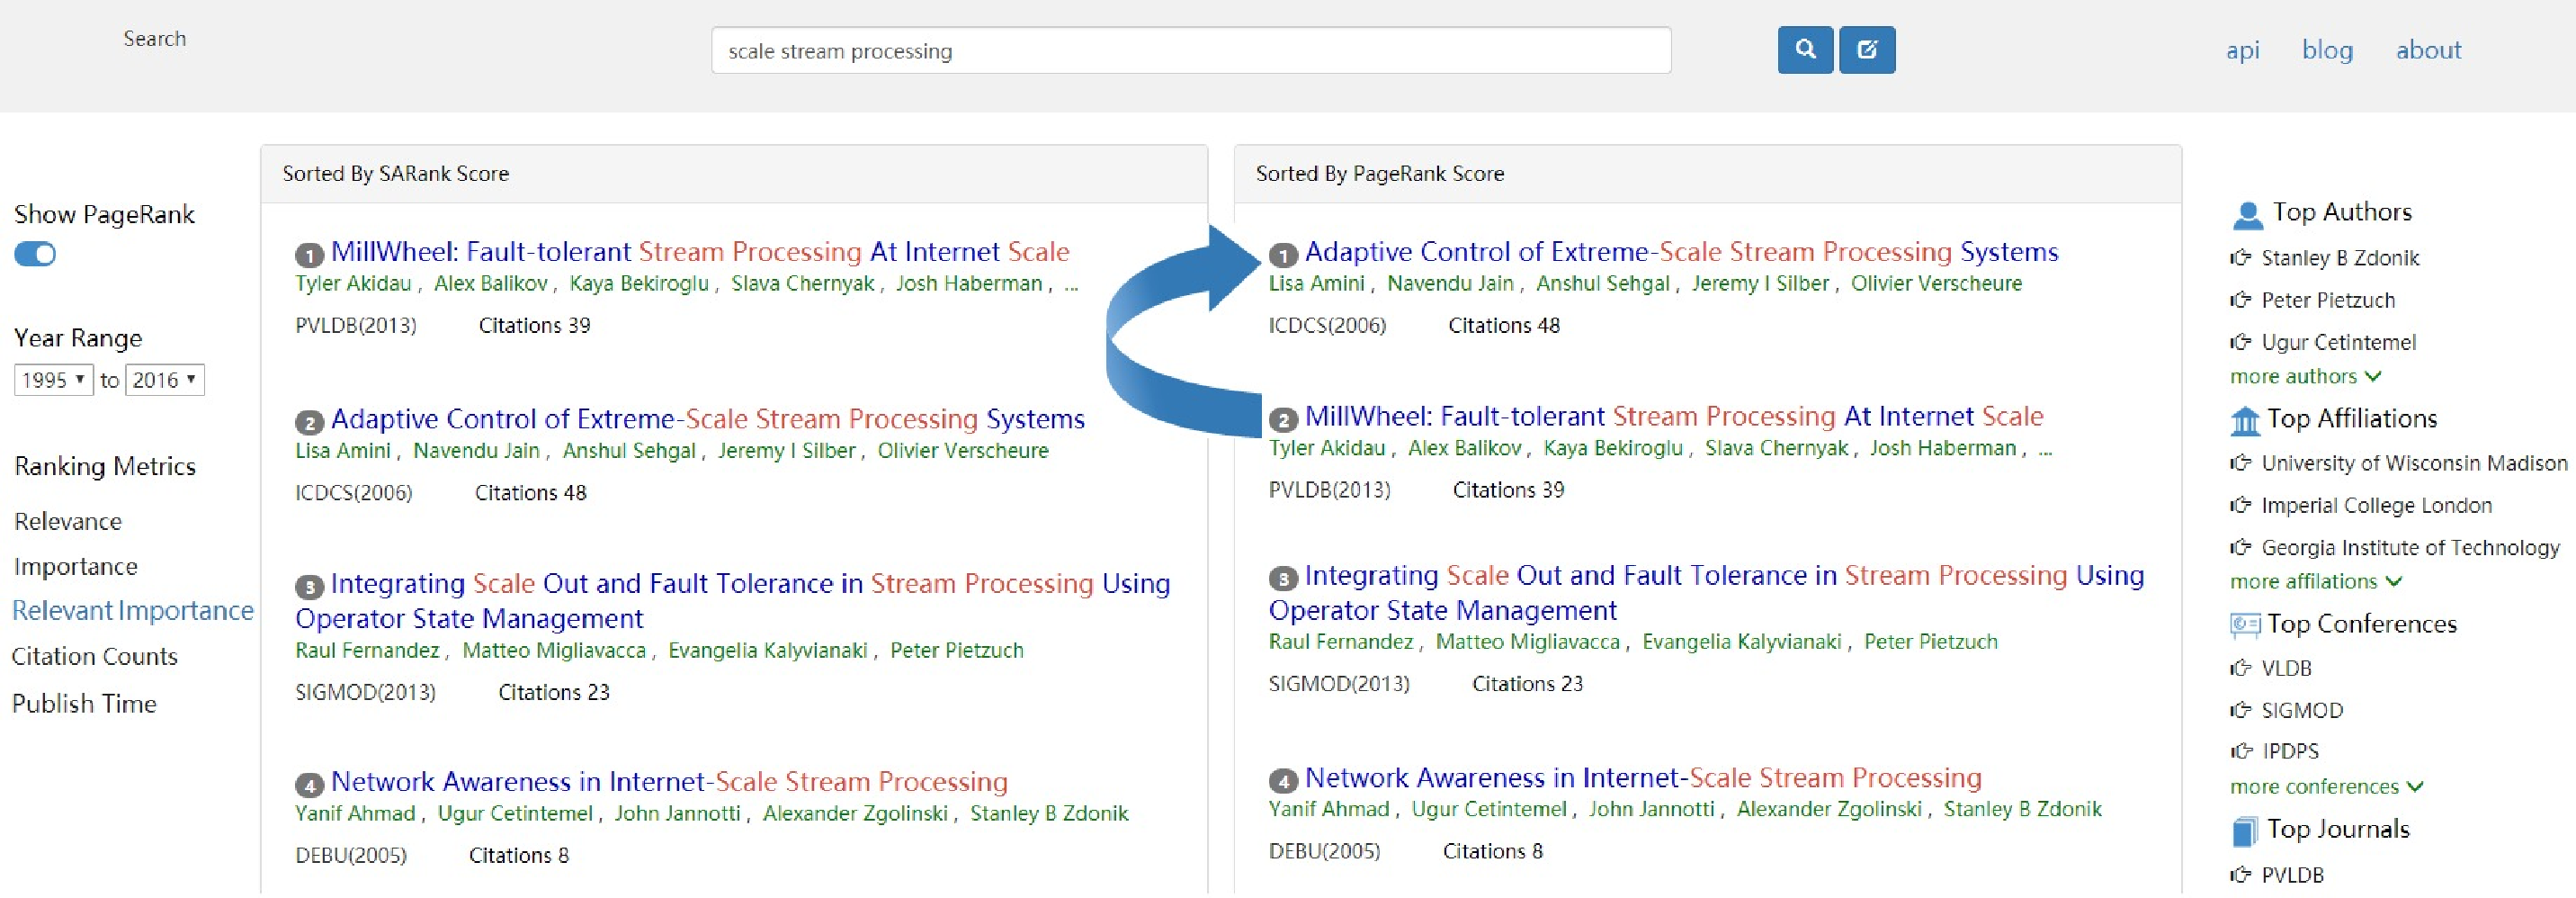
\includegraphics[width=\textwidth]{searchKeywords3.pdf}
\vspace{-3.5ex}
\caption{Demonstration of scholarly search and ranking quality evaluation}
\label{fig:searchKeywords}
\vspace{-2ex}
\end{figure*}

\marked{
We demonstrate our \oursystem system from four aspects: (1) scholarly search, (2) author profiling, (3) performance comparison between Neo4j and RDBMS MySQL and (4) ranking quality evaluation by case study. 
}

%The demonstration consists of three parts. (1) We walk through its various ranking metrics to demonstrate the ability of \oursystem to query and rank heterogeneous entities. (2) To further illustrate the profiling function based on scholarly data analysis, we take author profiling as an example. (3) In the scholarly information search scenario, we compare the query performance of MySQL and Neo4j through experiments.

\stitle{(1) Scholarly search}.
\marked{
Figure~\ref{fig:searchKeywords} presents the scholarly entity rankings under query ``scale stream processing".
The ranking metrics are displayed on the left-hand side. Note that \oursystem also supports queries within a specific range of years and displaying PageRank rankings.
When setting radio option checked and sorted by Relevant Importance, the rankings of articles sorted by  \sarank and PageRank score and the associated entities (authors, affiliations, conferences and journals) are shown in the middle and on the right-hand side.
Further, it is worth pointing out that users can also directly query entities by typing their names in the search box.
}


%Figure~\ref{fig:searchKeywords} presents the scholarly entity rankings under query ``scale stream processing".
%The ranking metrics are displayed on the left hand side. Note that \oursystem also supports queries within a specific range of years. 
%When sorted by relevant importance, the rankings of articles and the associated entities (authors, affiliations, journals and conferences) are shown in the middle and on the right hand side.
%Further, it is worth pointing out that users can also directly query entities by typing their names in the search box.
\begin{figure}
\centering
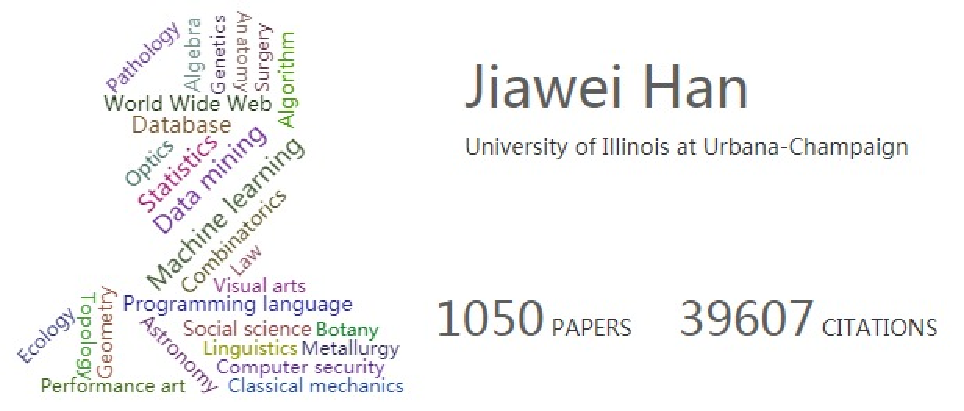
\includegraphics[width=0.98\columnwidth]{hjwAvatar.pdf}
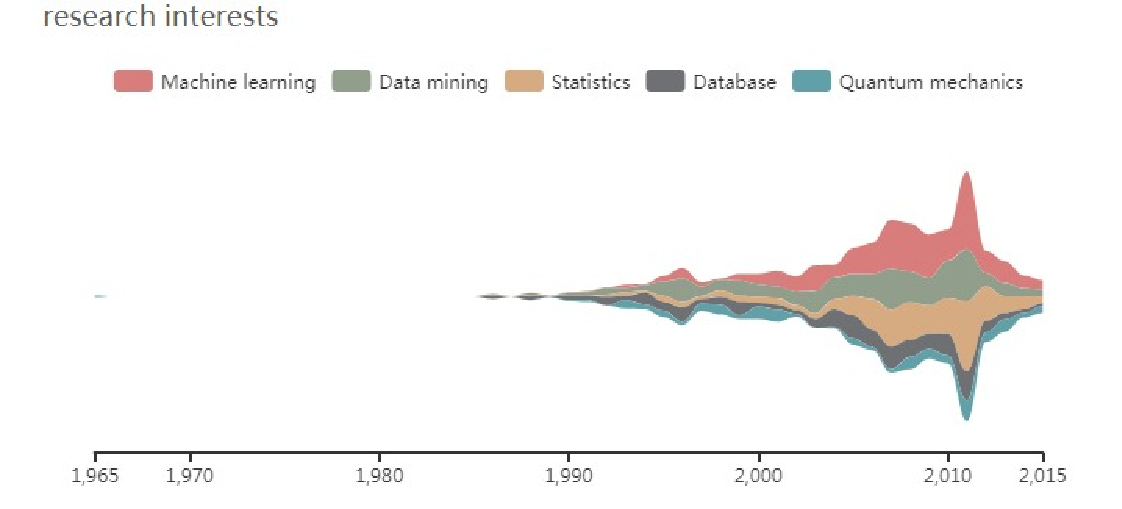
\includegraphics[width=\columnwidth]{hjwInterest.pdf}
%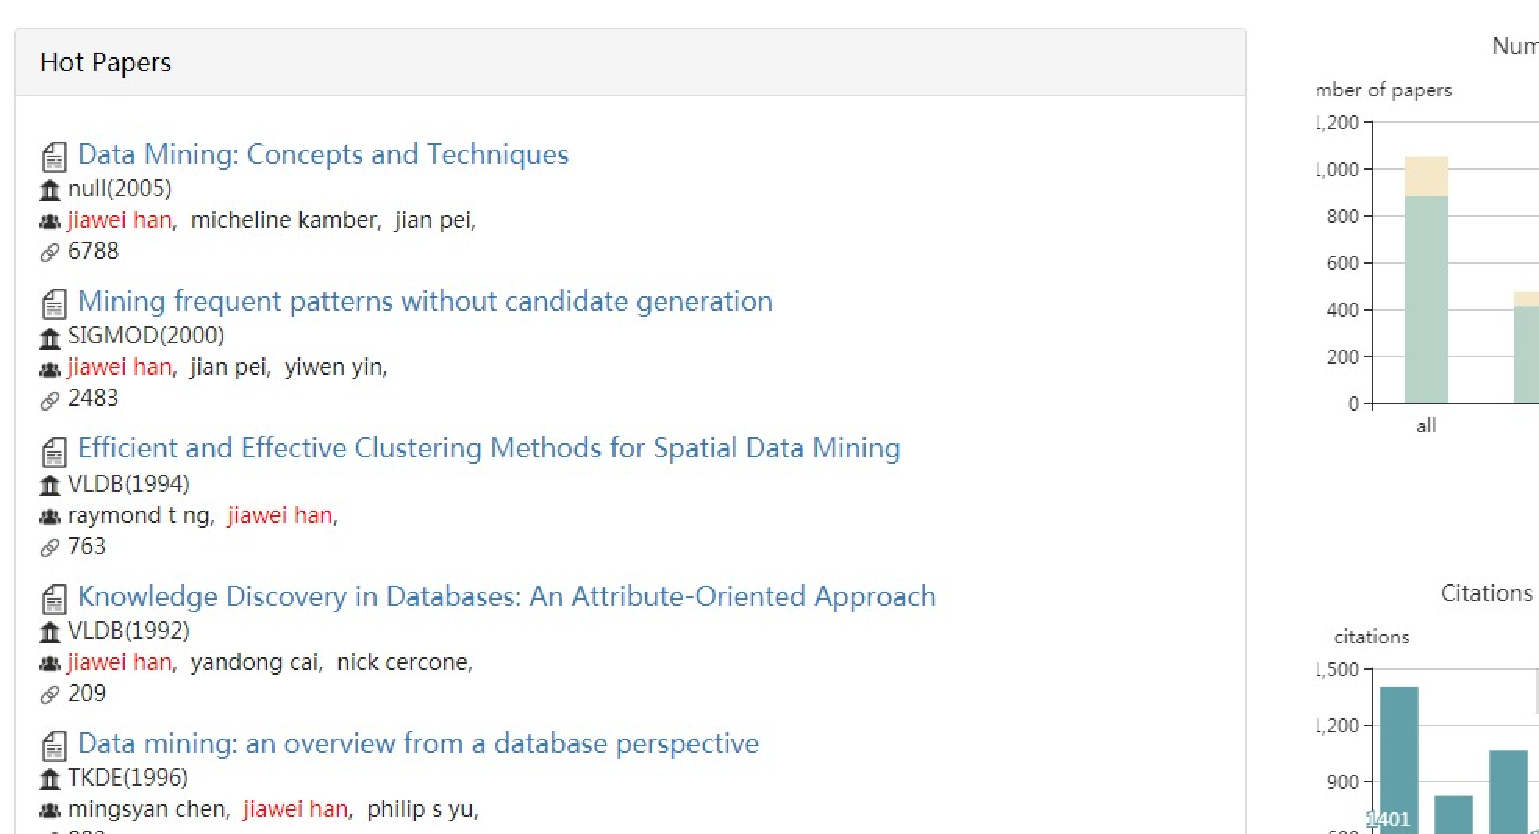
\includegraphics[width=\columnwidth]{hjwPapers.pdf}
\vspace{-3ex}
\caption{Demonstration of author profiling }
\label{fig:hjwProfile}
\vspace{-3.5ex}
\end{figure}




\stitle{(2) Author profiling}.
Figure~\ref{fig:hjwProfile} gives an example of author profiling for Prof. Jiawei Han.
First, the affiliation and number of published articles and citations are presented.
Second, a word cloud is given to summarize the author's fields of study, where the size of a word represents its importance in the author's research career. For instance, ``data mining'' and ``machine learning'' are identified as Prof. Jiawei Han's most important fields of study.
Third, \oursystem illustrates the details of the evolution of research interests, shown at the bottom of Fig.~\ref{fig:hjwProfile}, and users can find the relevant articles in each field of study.
Finally, functions such as co-authors analyses and statistics by times are provided in author profiling.

%Other functions in author profiling include co-author analysis and statistics by time. %We omit the demonstration of those functions due to space limitation.




\stitle{(3) Performance evaluation: Neo4j vs. MySQL}.
We compare the query performance of the adopted graph database Neo4j with traditional RDBMS MySQL. More specifically, we consider three types of queries, \ie (i) given an article ID, finding its title and authors, (ii)  given an article ID, finding its top--10 most important citations, and (iii) given an author ID, finding her/his published top--10 most important articles. Note that the numbers of joins are (2, 3, 4) for the three types of queries in MySQL, respectively.

We test a scenario for searching ``good'' articles. We randomly select 1000 articles and 100 authors whose citation counts and published articles are no less than 100 and 50, respectively, and compute the average processing time. As shown in Table~\ref{tab-compare}, Neo4j performs consistently faster than MySQL, which is on average (14.8\%, 19.4\%, 45.3\%) faster for the three types of queries.
Thus, structure-aware Neo4j is more efficient than MySQL for such scholarly analyses, especially for complex queries with more join operations.


\begin{table}[t!]
\begin{center}
\caption{Performance: Neo4j vs. MySQL}
%\vspace{-1ex}
\label{tab-compare}
\begin{scriptsize}

\begin{tabular}{|c|c|c|c|} %{lp{2cm}p{2cm}p{2cm}}
\hline
{Engines} & {Type I Queries} & {Type II Queries} & {Type III  Queries}\\
\hline %\hline
MySQL & 0.115 sec.  & 2.89 sec. & 3.60 sec. \\
\hline
Neo4j & 0.098 sec.  & 2.33 sec. & 1.97 sec. \\
\hline
\end{tabular}

\end{scriptsize}
\vspace{-4.5ex}
\end{center}
\end{table}

\stitle{(4) Ranking quality evaluation}.
\marked{
As shown in the middle of Figure~\ref{fig:searchKeywords}, we evaluate the ranking quality by comparing it with PageRank. Specifically, consider two articles: ``MillWheel: Fault-tolerant Stream Processing At Internet Scale"(millwheel) was published in PVLDB 2013 with 39 citations (ranked first in \sarank) and ``Adaptive Control of Extreme-Scale Stream Processing Systems" (adaptive) was published in ICDCS 2006 with 48 citations (ranked first in PageRank).}

\marked{
Although ``millwheel" has a little less citations, it gets published in PVLDB which has a higher impact than ICDCS. 
Moreover, ``millwheel" is published in 2013 later than ``adaptive" in 2006 as researchers potentially discover most recent influential articles.
Thus, ``millwheel" has a high influence and should be ranked first corresponding to \sarank. 
In concluding, \oursystem provide an effective ranking component for searching influential articles due to considering the temporal factor and assembling the article, venue and author entities.
}


\eat{
\stitle{Ranking Instance} We rank the conference papers \eg SIGMOD following the metrics of {\em time ranking}. We only collect articles published earlier than 2016, so the top of {\em time ranking} is the maximum importance score in 2015. As shown in fig. \ref{fig:sigmod}, we put ``Spark SQL: Relational Data Processing in Spark" in second place, which has the most citations(653) in SIGMOD 2015 up to now. More generally, in our top 10, there are 3 articles that has the most citation in SIGMOD 2015.
% the description in ICDE 2018

\par
Although they share the same venue component in the same year, the author of the article has higher prestige and popularity, such as Matei Zaharia and Michael Armbrust. Besides, an article in VLDB cites the paper published in the same years that increases the prestige and popularity of the citation components. Thus, the paper possesses a higher importance score by assembling the component of citation, author and venue.
}

